\usetikzlibrary{shapes,arrows}

\tikzstyle{input} = [coordinate]
\tikzstyle{output} = [coordinate]
\tikzstyle{block} = [draw, rectangle]
\tikzstyle{sum} = [draw, circle]

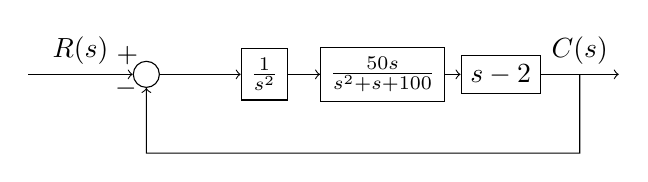
\begin{tikzpicture}[auto,node distance=1.5cm]
	% put the nodes (blocks, sums, etc..) where we want them
	\node [input,name=input] (in) {};
	\node [sum,right of=in] (sum1) {};
	\node [block,right of=sum1] (g1) {$\frac{1}{s^2}$};
	\node [block,right of=g1] (g2) {$\frac{50s}{s^2+s+100}$};
	\node [block,right of=g2] (g3) {$s-2$};
	\node [output,right of=g3] (out) {};

	% draw the feedforwards
	\draw [->] (in) -- node {$R(s)$} node[pos=0.95] {$+$} (sum1);
	\draw [->] (sum1) -- (g1);
	\draw [->] (g1) -- (g2);
	\draw [->] (g2) -- (g3);
	\draw [->] (g3) -- node[name=cs] {$C(s)$} (out);

	%h0 feedback
	\node[coordinate,below of=cs,node distance=1.3cm,name=p4] {}; 
	\node[coordinate,below of=sum1,node distance=1cm,name=p5] {};
	\draw [->] (cs) -- (p4) --  (p5) -- node[pos=0.99] {$-$} (sum1);

\end{tikzpicture}

